\section{Sintaxis}

La sintaxis de CSS está constituida por \textbf{selectores}, \textbf{propiedades} y \textbf{valores}. Veamos un simple ejemplo:
\begin{lstlisting}
    h1 {
        color: orange;
    }
\end{lstlisting}

Vemos que:
\begin{itemize}
    \item Hay una etiqueta HTML previo a la apertura de llaves, esta etiqueta es llamada \textbf{Selector}, que es la etiqueta destino a la cual se le aplicará un estilo.
    \item Una vez abiertas las llaves, hay una palabra, dos puntos y otra palabra, la primera es llamada \textbf{propiedad}, que básicamente es el atributo a estilizar de la etiqueta.
    \item Es llamado \textbf{valor} a la asignación de un dato o valor a la propiedad de un selector.
    \item \textbf{Un solo selector puede tener múltiples propiedades} a estilizar, cada una de ellas es separada mediante un \textbf{punto y coma} (\textbf{;}).
\end{itemize}


\subsection{Tipos de Selectores}

Primero, debemos aclarar dos conceptos o atributos de etiqueta HTML que se verán muy constantemente a lo largo del desarrollo de sitios web:
\begin{itemize}
    \item El atributo \textbf{id} permite asignarle un identificador a una etiqueta, este identificador es utilizado por CSS para aplicar un estilo particular.
    \item El atributo \textbf{class} opera de la misma manera que \textbf{id}, la diferencia radica en que i\textit{d} se limita a un solo uso por página, mientras que \textit{class} puede usarse múltiples veces, te preguntarás porqué, la respuesta está en que JavaScript utiliza también la palabra \textit{id} en su sintaxis, por lo que, si utilizará un estilo en múltiples etiquetas, se recomienda utilizar \textbf{class}.
    \item El orden de prioridad de selectores es:
    \begin{enumerate}
        \item id.
        \item class.
        \item type.
    \end{enumerate}
\end{itemize}
\begin{itemize}
    \item \textbf{Regular}: se le aplica un estilo a una etiqueta.
    \item \textbf{id \& class}: se le aplica un estilo a un \textbf{identificador} (\textbf{id}) o \textbf{class} especifico mediante el caracter \textbf{gato} (\textbf{\#}) y \textbf{punto} (\textbf{.}) respectivamente
\end{itemize}

Veamos un ejemplo (\textit{Figura \ref{fig: 1}}):
\begin{lstlisting}
estilos.css
    p {
        color: white;
        background-color: gray;
    }
    #intro {
        background-color: red;
    }
    .cuerpo {
        background-color: green;
    }

prueba.html
    <p>Párrafo 1</p>
    <p class="cuerpo">Párrafo 2</p>
    <p class="cuerpo" id="intro">Párrafo 3</p>
    <div class="cuerpo" id="intro">
        <p>Párrafo 4</p>
    </div>
\end{lstlisting}
\begin{figure}[H]
    \begin{center}
        \caption{Orden de prioridad de estilos}
        \label{fig: 1}
        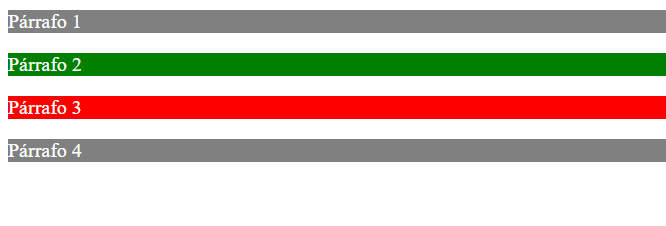
\includegraphics[width=12cm]{ss/tipos de estilos.png}
    \end{center}
\end{figure}

Vemos que hay cuatro párrafos, a cada uno tiene un estilo diferente: el párrafo 1 no tiene ni identificador ni clase, por lo que el estilo a aplicar es el de las etiquetas \textbf{p}; el párrafo 2 tiene el identificador "intro", por lo que el estilo a aplicar es el de dicho identificador; el párrafo 3 tiene la clase "cuerpo", por lo que el estilo a aplicar es el de dicha clase; el párrafo 4 está contenido dentro de una etiqueta \textbf{div}, la cual tiene el identificador y clase anteriormente mencionados, por lo que debemos considerar el orden de prioridad de los selectores CSS y HTML, por lo que el estilo a aplicar es el de las etiquetas \textbf{p}.


\subsection{Selectores descendentes}

Podemos aplicar un estilo a una etiqueta contenida dentro de otra que posee un estilo definido (un identificador, una clase o estilo de etiqueta), es decir, clase dentro de clase, identificador dentro de un identificador, clase dentro de identificador o viceversa, miremos un ejemplo (\textit{Figura \ref{fig: 2}}):
\begin{lstlisting}
estilos.css
    #intro .primero em {
        color: pink;
        background-color: gray;
    }

prueba.html
    <div id="intro">
        <p class="primero"><em>Párrafo 1</em> dentro del div</p>
    </div>
    <p class="primero">Párrafo 2 fuera del div.</p>
    <p>Párrafo 3 fuera del div</p>
\end{lstlisting}
\begin{figure}[H]
    \begin{center}
        \caption{Selectores descendentes}
        \label{fig: 2}
        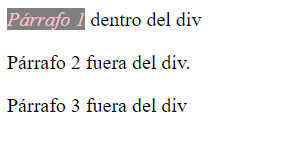
\includegraphics[width=6cm]{ss/selectores descendente.png}
    \end{center}
\end{figure}


\subsection{Comentarios}

Para comentar una o varias líneas de código en CSS se debe escribir los caracteres \textbf{/*} al comienzo o primer línea y \textbf{*/} al final o última línea de código.
\begin{lstlisting}
    /* Esto es un comentario. */

    /* Todo este estilo está comentado.
    p {
        color: red;
    } */
    
    #intro .primero em {
    color: pink;
    background-color: gray;
}
\end{lstlisting}



\section{Formas de aplicar estilos CSS}

Los estilos CSS pueden ser aplicados de tres maneras sencillas:


\subsection{Inline}

Implica aplicar el estilo mediante la atributo HTML \textbf{style}, dentro de sus dos comillas, asignamos las propiedades CSS de estilo que la etiqueta u objeto HTML tendrá, únicamente esta etiqueta, no el resto del mismo tipo.
\begin{lstlisting}
    <html>
        <head>
            <title>Prueba</title>
        </head>
        <body>
            <!-- Estilo Inline. -->
            <p style="color: white; background-color: gray;">Hola </p>
            <p>mundo.</p>
        </body>
    </html>
\end{lstlisting}

En el ejemplo anterior, solamente la primer etiqueta tendría un estilo definido.


\subsection{Embedded o Internal}

Contrario a la forma \textit{Inline}, donde se le aplica un estilo a una sola etiqueta, la forma \textbf{Embedded} crea un estilo dentro de la estructura HTML y se le puede aplicar a cuantas etiquetas se desee. Estos estilos internos son creados en la cabecera de la estructura del documento, utilizando la etiqueta \textbf{style}.
\begin{lstlisting}
    <html>
        <head>
            <title>Prueba</title>
            <!-- Estilo Embedded. -->
            <style>
                p {
                    color: white;
                    background-color> gray;
                }
            </style>
        </head>
        <body>
            <p>Hola </p>
            <p>mundo.</p>
        </body>
    </html>
\end{lstlisting}

En el ejemplo anterior, ambas etiquetas \textbf{p} tienen un mismo estilo definido. Es recomendable utilizar estilos internos cuando una sola página de un sitio web tiene un estilo único.


\subsection{External}

Con este método, debemos contar con un archivo con extensión \textbf{.css} en nuestro directorio y lo enlazamos a nuestro documento HTML mediante la siguiente etiqueta:
\begin{center}
    \textit{<link href="ejemplo.css" rel="stylesheet">}
\end{center}

Veamos un ejemplo:
\begin{lstlisting}
/* Estilo External. */
ejemplo.css
    p {
        color: white;
        background-color: gray;
    }

prueba.html
    <html>
        <head>
            <title>Prueba</title>
            <!-- Enlaza hoja de estilos al documentl HTML. -->
            <link href="ejemplo.css" rel="stylesheet">
        </head>
        <body>
            <p>Hola </p>
            <p>mundo </p>
            <p>estoy probando estilos CSS.</p>
        </body>
    </html>
\end{lstlisting}

Así, todos los cambios que hagamos a la hoja de estilos en su propio archivo se verá reflejado en el sitio web, siempre y cuando esta hoja de estilos esté ligada a la página.



\section{Herencia}

Al igual que otros lenguajes con un enfoque distinto, CSS aplica herencia a los elementos o etiquetas contenidas dentro de una que ya tenga un estilo definido, veamos como funciona esto:
\begin{lstlisting}
estilos.css
    body {
        color: red;
    }

prueba.html
    <p>Hola </p>
    <p>mundo </p>
    <p>estoy probando estilos CSS.</p>
\end{lstlisting}

En el ejemplo, ninguna etiqueta \textbf{p} tiene estilo definido, por lo que se les aplica el estilo de su etiqueta padre \textbf{body}.
\begin{lstlisting}
estilos.css
    body {
        color: red;
    }
    p {
        color: blue;
    }

prueba.html
    <p>Hola </p>
    <p>mundo </p>
    <p>estoy probando estilos CSS.</p>
\end{lstlisting}

Se creamos un estilo para las etiquetas \textbf{p} con un color de texto distinto, a estas etiquetas se les aplicará el estilo diseñado para ellas, en vez del estilo de su padre \textbf{body}, por lo que podemos concluir que \textbf{los estilos de los hijos de etiquetas tienen prioridad sobre sus padres}.
